% !TeX root = er.tex

\chapter{Control}\label{ch.control}

Os algoritmos de robótica tomam decisões. O robô recebe uma tarefa, mas para realizar a tarefa ele deve tomar ações e estas ações dependem do ambiente, conforme detectado pelos sensores. Por exemplo, se um robô quiser trazer um objeto de uma prateleira em um armazém para uma pista de entrega, ele deve usar sensores para navegar até a prateleira apropriada, para detectar e agarrar o objeto, e então navegar de volta para o caminhão e carregar o objeto. Somente robôs que atuam em ambientes extremamente bem definidos podem realizar tais tarefas sem a informação dos sensores. Um exemplo é um braço robótico montando um dispositivo em uma fábrica; se as peças estiverem precisamente posicionadas na superfície de trabalho, o robô pode manipular as peças sem detectá-las. Mas, na maioria dos ambientes, os sensores devem ser usados. Em um armazém pode haver obstáculos no caminho até a prateleira, o objeto não será posicionado com precisão na prateleira e o caminhão nunca será estacionado exatamente no mesmo lugar. O robô precisa se adaptar a estas pequenas variações usando \emph{algoritmos de controle} para tomar decisões: com base nos dados dos sensores, que ações o robô precisa realizar para realizar a tarefa? Existe uma sofisticada teoria matemática de controle que é fundamental na robótica. Neste capítulo, apresentamos os conceitos básicos dos algoritmos de controle.

A seção~\ref{s.control-model} explica a diferença entre dois modelos de controle: controle de malha aberta onde os parâmetros do algoritmo são definidos com antecedência e controle de malha fechada onde os dados dos sensores influenciam o comportamento do algoritmo. As seções~\ref{s.on-off}--\ref{s.pid} apresentam quatro algoritmos de controle de malha fechada cada vez mais sofisticados. O projetista de um robô deve escolher entre estes e outros algoritmos similares para selecionar aquele que oferece o desempenho adequado pelo menor custo computacional.

\section{Modelos de controle}\label{s.control-model}

Há duas maneiras que um algoritmo de controle pode decidir sobre uma ação. Em um sistema de circuito aberto, os parâmetros do algoritmo de controle são predefinidos e não mudam enquanto o sistema funciona. Em um sistema de circuito fechado, os sensores medem o erro entre o estado desejado do sistema e seu estado real, e este erro é usado para decidir que ação tomar.

\subsection{Controle de circuito aberto}

Uma torradeira é uma máquina que realiza ações semi-autônomas. Você coloca fatias de pão na torradeira, ajusta o temporizador e empurra a alavanca para baixo para iniciar a ação de torrar. Como todos sabemos, os resultados não são garantidos: se a duração do temporizador for muito curta, temos que torrar o pão novamente; se a duração do temporizador for muito longa, o cheiro de torrada queimada flutua através da cozinha. O resultado é incerto porque uma torradeira é um \emph{sistema de controle de laço aberto}. Ele não verifica o resultado da ação do torrador para ver se o resultado necessário foi alcançado. Os sistemas de circuito aberto são muito familiares: em uma máquina de lavar você pode ajustar a temperatura da água, a duração do ciclo e a quantidade de detergente utilizada, mas a máquina não mede a "limpeza" da roupa (o que quer que isso signifique) e modifica suas ações de acordo.

Um robô móvel que se desloca para uma posição alvo baseada apenas na odometria (Sect.~\ref{s.odometry}) também está utilizando o controle de malha aberta. Ao controlar a potência do motor e a duração do funcionamento dos motores, o robô pode calcular a distância que se moveu. No entanto, variações na velocidade das rodas e na superfície sobre a qual o robô se move causarão incerteza na posição final do robô. Na maioria das aplicações, a odometria pode ser usada para mover o robô para as proximidades da posição de objetivo, ponto em que são usados sensores para mover o robô para a posição exata de objetivo, por exemplo, usando sensores para medir a distância até um objeto.

\subsection{Controle de circuito fechado}

Para alcançar um comportamento autônomo, os robôs utilizam \emph{sistemas de controle de loop fechado}. Já encontramos sistemas de circuito fechado nos veículos Braintenberg (Activity~\ref{act.attractive}):
\begin{quote}
\normalsize\noindent\textbf{Especificação (Atrativo e repulsivo):} Quando um objeto se aproxima do robô por trás, ele foge até ficar fora de alcance.
\end{quote}
O robô deve \emph{medir} a distância até o objeto e parar quando essa distância for suficientemente grande. O ajuste de potência dos motores depende da medição da distância, mas o robô se move a uma velocidade que depende da potência dos motores, o que muda a distância até o objeto, o que novamente modifica o ajuste de potência, o que faz com que o robô se mova a uma velocidade que depende da potência dos motores, o que muda a distância até o objeto, o que novamente modifica o ajuste de potência, \ldots. Este comportamento circular é a origem do termo "loop fechado".

Agora formalizamos a especificação de um sistema de controle de loop fechado para um robô (Fig.~\ref{fig.control-model}). A variável $r$ representa o valor \emph{reference value}, a especificação da tarefa do robô. Em um robô de armazém, os valores de referência incluem a posição do robô em relação a uma pilha de prateleiras e a distância do braço da pinça em relação ao objeto a ser pego. Um valor de referência não pode ser usado diretamente pelo robô; ao invés disso, ele deve ser transformado em um valor \emph{control value} $u$. Por exemplo, se o valor de referência for a posição do robô em relação a uma prateleira, o valor de controle será a potência dos motores e a duração que os motores estão em funcionamento. A variável $y$ representa a saída, ou seja, o estado real do robô, por exemplo, a distância até um objeto.

\begin{figure}
\begin{center}
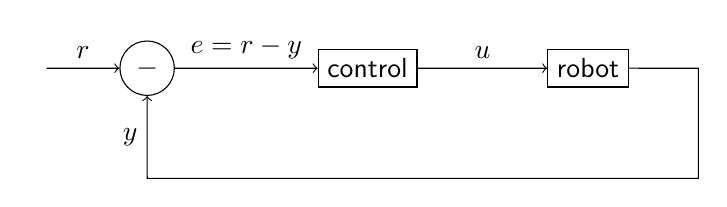
\begin{tikzpicture}[scale=1.4]
\node (input) at (0,1) {};
\node[circle,draw] (diff) at (1,1) {$-$};
\node[rectangle,draw] (control) at (3,1) {\textsf{control}};
\node[rectangle,draw] (robot) at (5,1) {\textsf{robot}};
\draw[->] (input) -- node[above] {$r$} (diff);
\draw[->] (diff)  -- node[above] {$e=r-y$} (control);
\draw[->] (control) -- node[above] {$u$} (robot);
\draw[->] (robot) -- ++(1,0) -- ++(0,-1) -- ++(-5,0) -- node[left] {$y$} (diff);
\end{tikzpicture}
\caption{Um sistema de controle de circuito fechado}\label{fig.control-model}
\end{center}
\end{figure}

O modelo na Fig.~ref{fig.control-model} também é chamado de \emph{feedback control system}, porque o valor de saída $y$ é alimentado pelo algoritmo de controle e usado para calcular o valor de controle. A saída é comparada com o valor de referência para computar $e=r-y$, o \emph{error}. O algoritmo de controle usa o erro para gerar o sinal de controle $u$, que é a entrada para o robô.

\subsection{O período de um algoritmo de controle}

Algoritmos de controle são executados periodicamente (Algoritmo~\ref{alg.control-loop}). O software do robô inicializa uma variável \emph{timer} para a duração necessária do período de execução do algoritmo, por exemplo, a cada $20$ ms. O computador embutido tem um \emph{relógio de hardware} que ``fixa'' em intervalos fixos, causando uma interrupção. A interrupção é tratada pelo sistema operacional que decreta o valor da variável temporizador. Quando o valor desta variável chega a zero, o timer expira e um evento é levantado no software causando a execução do algoritmo de controle.

\begin{figure}
\begin{alg}{Esboço do algoritmo de controle}{control-loop}
\hline
&\idv{}integer period&// Duration of timer period\\
&\idv{}integer timer&// Timer variable\\
\hline
\stl{}&period \ass $\cdots$&// Period in milliseconds\\
\stl{}&timer \ass period&// Initialize the timer\\
\stl{}&loop&\\
\stl{}&\idc{}when timer-expired-event occurs&\\
\stl{}&\idc{}\idc{}control algorithm&// Run the algorithm\\
\stl{}&\idc{}\idc{}timer \ass period&// Reset the timer\\
\hline\hline
&// {\bfseries Operating system}&\\
\stl{}&when hardware-clock-interrupt occurs&\\
\stl{}&\idc{} timer \ass timer $-$ $1$&// Decrement the timer\\
\stl{}&\idc{} if timer $=$ $0$&// If the timer expires\\
\stl{}&\idc{}\idc{} raise timer-expired-event&// \ \ \ \ raise an event\\
\end{alg}
\end{figure}

O período do algoritmo é um parâmetro importante no projeto de um sistema de controle. Se o período for muito curto, recursos computacionais valiosos serão desperdiçados e o computador pode ficar sobrecarregado ao ponto de os comandos para o robô chegarem tarde demais. Se o período for muito longo, o robô não responderá a tempo para corrigir erros em seu movimento.

\smallskip

\noindent\textbf{Exemplo} Considere um robô se aproximando de um objeto que está a $10$ cm de distância a $2$ cm/s. Um período de controle de $1$ ms desperdiçaria recursos computacionais porque o robô moverá apenas $0,002$ cm ($0,02$ mm) durante o ciclo de $1$ ms do algoritmo de controle. Mudanças na potência do motor em distâncias tão pequenas não afetarão a capacidade do robô de cumprir sua tarefa. No extremo oposto, um período de controle de $2$ s é ainda pior: o robô moverá $4$ cm durante este período e provavelmente colidirá com o objeto. Um período de controle de aproximadamente $0,25$ s ($250$ ms) durante o qual o robô se move $0,5$ cm parece um valor razoável para começar, pois $0,5$ cm é uma distância que é significativa em termos de aproximação de um objeto. Você pode experimentar períodos em torno deste valor para determinar o período ideal: um que alcance um comportamento satisfatório com um período o mais longo possível para reduzir o custo do cálculo.

\begin{framed}
\act{Definição do período de controle}{setperiod}
\begin{itemize}
\item No exemplo, chegamos à conclusão de que o período ótimo do algoritmo de controle foi da ordem de décimos de segundo. Nesta atividade, perguntamos qual deveria ser o período ótimo para outros algoritmos de controle.
\item Um sistema de aquecimento doméstico contém um termostato para controlar a temperatura. Qual seria o período ideal para o algoritmo de controle? O período depende dos parâmetros de engenharia do sistema de aquecimento e das propriedades físicas de como o calor é transferido para as salas. Explique como medir esses fatores e como eles afetam o período de controle.
\item Considere um carro que se auto dirige tentando estacionar. Que suposições você precisa fazer para projetar um período de controle? O que seria um período razoável?
\item Como as propriedades dos sensores afetam o período de controle? Para o exemplo de um robô se aproximando de um objeto, como o período mudaria se o sensor pudesse detectar o objeto a $2$ cm, $5$ cm, $10$ cm, $20$ cm, $40$ cm?
\end{itemize}
\end{framed}

Definimos agora uma seqüência de quatro algoritmos de controle, cada um deles construindo sobre o anterior e proporcionando um controle mais preciso, ao preço de uma maior complexidade computacional. Na prática, o projetista do sistema deve escolher o algoritmo mais simples que permita que o robô cumpra sua tarefa.

Os algoritmos são apresentados no contexto de um robô que deve se aproximar de um objeto e parar a uma distância de $s$ em frente a ele. A distância é medida por um sensor de proximidade e a velocidade do robô é controlada através do ajuste da potência dos motores.


\section{Controle on-off}\label{s.on-off}


O primeiro algoritmo de controle é chamado de algoritmo \emph{on-off} ou \emph{bang-bang} (Algoritmo~\ref{alg.onoff}). Definimos uma constante \p{referência} que é a distância na frente do objeto no qual o robô deve parar. A variável \p{medida} é a distância real medida pelo sensor de proximidade. O \p{erro} é a diferença entre os dois:
\begin{center}
\p{error} $\leftarrow$ \p{reference} $-$ \p{measured},
\end{center}
que é negativo se o robô estiver muito longe do objeto e positivo se estiver muito próximo do objeto. As potências do motor são viradas para frente ou para trás, dependendo do sinal do erro. Por exemplo, se a distância de referência for $10$ cm e a distância medida for $20$ cm, o robô está muito distante e o erro é $10$ cm. Portanto, os motores devem ser ajustados para avançar.
\begin{figure}
\begin{alg}{On-off controller}{onoff}
&\idv{}integer reference \ass $\cdots$&// Reference distance\\
&\idv{}integer measured &// Measured distance\\
&\idv{}integer error &// Distance error\\
\hline
\stl{}&error \ass reference $-$ measured&\\
\stl{}&if error $<$ 0&\\
\stl{}&\idc{} left-motor-power \ass $100$&// Move forwards\\
\stl{}&\idc{} right-motor-power \ass $100$&\\
\stl{}&if error $=$ 0&\\
\stl{}&\idc{} left-motor-power \ass $0$&// Turn off motors\\
\stl{}&\idc{} right-motor-power \ass $0$&\\
\stl{}&if error $>$ 0&\\
\stl{}&\idc{} left-motor-power \ass $-100$&// Move backwards\\
\stl{}&\idc{} right-motor-power \ass $-100$&\\
\end{alg}
\end{figure}

O robô se aproxima do objeto em velocidade máxima. Quando o robô atinge a distância de referência do objeto, leva tempo para que o sensor seja lido e o erro seja computado. Mesmo que o robô meça uma distância exatamente igual à distância de referência (o que é improvável), o robô não será capaz de parar imediatamente e irá ultrapassar a distância de referência. O algoritmo então fará com que o robô volte à velocidade máxima, passando novamente a distância de referência. Quando o timer faz com que o algoritmo de controle seja executado novamente, o robô inverterá a direção e seguirá em frente a toda velocidade. O comportamento resultante do robô é mostrado na Fig.~\ref{fig.onoff}: o robô irá oscilar em torno da distância de referência ao objeto. É altamente improvável que o robô realmente pare na distância de referência ou próximo a ela.

\begin{figure}
\begin{center}
\begin{tikzpicture}[scale=1.2]
\draw[<->] (0,5) -- node[sloped,above,rotate=180] {\p{distance}} (0,0) node[left] {} -- node[below] {\p{time}} (8,0);
\draw (0,2) node[below right] {$r$} -- (8,2);
\draw[thick] plot coordinates {(0,5) (2,1.5) (3,2.5) (4,1.5) (5,2.5) (6,1.5)(7,2.5) (8,1.5)};
\end{tikzpicture}
\caption{Comportamento do algoritmo on-off}\label{fig.onoff}
\end{center}
\end{figure}

Uma desvantagem adicional do algoritmo on-off é que a inversão de direção freqüente e abrupta resulta em altas acelerações. Se estivermos tentando controlar um braço de garra, os objetos que ele está carregando podem ser danificados. O algoritmo gera altos níveis de desgaste nos motores e em outras partes móveis mecânicas.

\begin{framed}
\act{Controlador on-off}{onoff}
\begin{itemize}
\item Implemente o algoritmo on-off em seu robô para a tarefa de parar a uma distância de referência de um objeto.
\item Execute-o várias vezes a partir de distâncias diferentes do objeto.
\item O Algoritmo do item Algoritmo Ref (amálgama de amálgama de ligamento) pára o robô quando o erro é exatamente zero. Modifique a implementação para que o robô pare se o erro estiver dentro de uma pequena distância em torno de zero. Experimente com faixas diferentes e veja como elas afetam o comportamento do robô.
\end{itemize}
\end{framed}

\section{Controlador proporcional (P)}\label{s.p}

Para desenvolver um algoritmo melhor, nos inspiramos em andar de bicicleta. Suponha que você esteja andando de bicicleta e veja que o semáforo à sua frente ficou vermelho. Você não espera até o último momento quando estiver na linha de parada e depois aperta com força a alavanca do freio; se fizer isso, você pode ser atirado da bicicleta! O que você faz é diminuir sua velocidade gradualmente: primeiro, você pára de pedalar; depois, você aperta o freio suavemente para diminuir um pouco mais a velocidade; finalmente, quando você está na linha de parada e vai devagar, você aperta com mais força para parar completamente a bicicleta. O algoritmo usado por um ciclista pode ser expresso como:
\begin{quote}
\normalsize\noindent{}Reduza mais sua velocidade à medida que você se aproxima da distância de referência.
\end{quote}
A diminuição da velocidade é (inversamente) \emph{proporcional} ao quão próximo você está do semáforo: quanto mais próximo você está, mais você abranda. O fator de proporcionalidade é chamado de \emph{ganho} do algoritmo de controle. Uma maneira alternativa de expressar este algoritmo é:
\begin{quote}
\normalsize\noindent{}Reduza mais sua velocidade à medida que o erro entre a distância de referência e a distância medida fica menor.
\end{quote}

Algoritmo~\ref{alg.proportional} é o \emph{algoritmo de controle proporcional} ou um \emph{P-controlador}.

\begin{figure}
\begin{alg}{Controlador proporcional}{proportional}
&\idv{}integer reference \ass $\cdots$&// Reference distance\\
&\idv{}integer measured &// Measured distance\\
&\idv{}integer error &// Error\\
&\idv{}float gain \ass $\cdots$& // Proportional gain\\
&\idv{}integer power & // Motor power\\
\hline
\stl{}&error \ass reference $-$ measured&// Distances\\
\stl{}&power \ass gain * error&// Control value\\
\stl{}&left-motor-power \ass power&\\
\stl{}&right-motor-power \ass power&\\
\end{alg}
\end{figure}

\smallskip

\noindent\textbf{Exemplo} Suponha que a distância de referência é $100$ cm e o ganho é $-0,8$. Quando o robô está a $150$ cm do objeto, o erro é $100-150=-50$ e o algoritmo de controle ajustará a potência para $-0,8\cdot -50=40$. A tabela~\ref{tab.p-controller} mostra os erros e as configurações de potência para três distâncias. Se o robô ultrapassar a distância de referência de $100$ cm e uma distância de $60$ cm for medida, a potência será ajustada para $-32$ fazendo com que o robô se mova para trás.

\begin{table}
\caption{Controlador proporcional para ganho de $-0.8$}
\label{tab.p-controller}
\begin{tabular}{rrr}
\hline\noalign{\smallskip}
\multicolumn{1}{c}{distância} & \multicolumn{1}{c}{\ \ \ erro}& \multicolumn{1}{c}{\ \ \ energia}\\
\noalign{\smallskip}\hline\noalign{\smallskip}
$150$ & $-50$ & $40$\\
$125$ & $-25$ & $20$\\
$60$ & $40$ & $-32$\\
\noalign{\smallskip}\hline\noalign{\smallskip}
\end{tabular}
\end{table}

Figura~\ref{fig.p-control} traça a distância do robô ao objeto como uma função do tempo quando o robô é controlado por um controlador P. A linha rotulada $r$ é a distância de referência. A mudança na potência do motor é suave para que o robô não experimente acelerações e desacelerações rápidas. A resposta é um pouco lenta, mas o robô se aproxima da distância alvo.

\begin{figure}
\begin{center}
\begin{tikzpicture}[scale=1.2]
\draw[<->] (0,5) -- node[sloped,above,rotate=180] {\p{distance}} (0,0) node[left] {} -- node[below] {\p{time}} (8,0);
\draw (0,1.9) node[below right] {$r$} -- (8,1.9);
\draw[domain=0:8,samples=100,thick] plot (\x,{3*exp(-2*\x)+2});
\end{tikzpicture}
\caption{Comportamento do controlador P}\label{fig.p-control}
\end{center}
\end{figure}

Infelizmente, o robô não atinge realmente a distância de referência. Para entender porque isto acontece, considere o que acontece quando o robô está muito próximo da distância de referência. O erro será muito pequeno e, conseqüentemente, a potência será muito baixa. Em teoria, o ajuste de baixa potência deve fazer com que o robô se mova lentamente, eventualmente alcançando a distância de referência. Na prática, a potência do motor pode se tornar tão baixa que não será capaz de superar o atrito interno nos motores e sua conexão com as rodas, de modo que o robô pare de se mover.

Pode parecer que aumentar o ganho do controlador P poderia superar este problema, mas um ganho alto sofre de uma séria desvantagem. A figura~\ref{fig.gain} mostra o efeito do ganho no controlador P. O ganho maior (linha vermelha tracejada) faz com que o robô se aproxime mais rapidamente da distância de referência, enquanto o ganho menor (linha azul tracejada) faz com que o robô se aproxime mais lentamente da distância de referência. Entretanto, se o ganho for muito alto, o controlador P funciona como um controlador on-off com uma resposta oscilante (linha verde). Dizemos que o controlador é \emph{unstable}.

\begin{figure}
\begin{center}
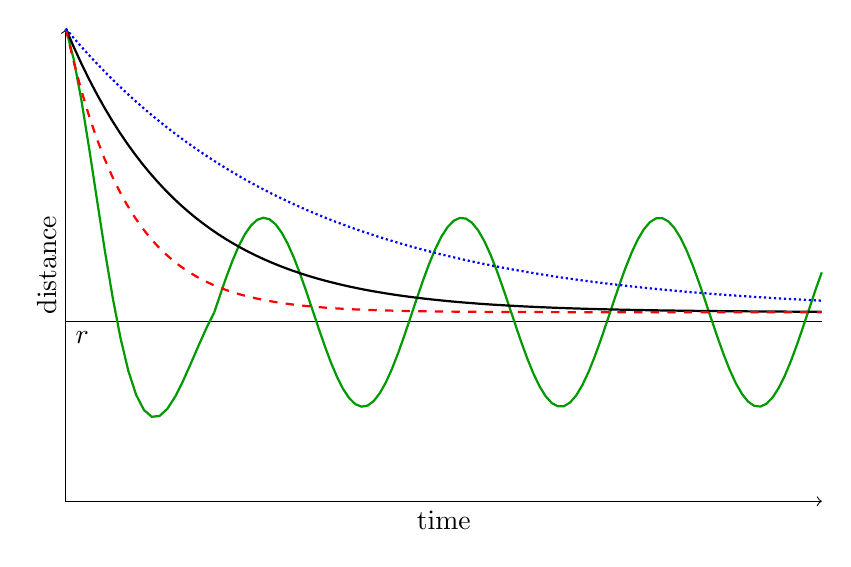
\begin{tikzpicture}[scale=1.2]
\draw[<->] (0,5) -- node[sloped,above,rotate=180] {\p{distance}} (0,0) node[left] {} -- node[below] {\p{time}} (8,0);
\draw (0,1.9) node[below right] {$r$} -- (8,1.9);
\draw[domain=0:1.57,samples=20,thick,green!60!black] plot (\x,{3*exp(-\x)*cos(3*\x r)+2});
\draw[domain=1.57:8,samples=100,thick,green!60!black] plot (\x,{cos(3*\x r)+2});
\draw[domain=0:8,samples=100,thick] plot (\x,{3*exp(-.8*\x)+2});
\draw[domain=0:8,samples=100,dashed,red,thick] plot (\x,{3*exp(-1.5*\x)+2});
\draw[domain=0:8,samples=100,densely dotted,blue,thick] plot (\x,{3*exp(-.4*\x)+2});
\end{tikzpicture}
\caption{O efeito do ganho no controlador P: ganho menor (linha azul tracejada), ganho maior (linha vermelha tracejada), ganho excessivo (linha verde oscilante)}\label{fig.gain}
\end{center}
\end{figure}

Há situações em que o controlador P não pode alcançar a distância de referência mesmo em um sistema ideal. Suponha que o objeto em si esteja se movendo a uma velocidade constante para longe do robô. O controlador P ajustará a potência máxima do motor para fazer com que o robô se mova rapidamente em direção ao objeto. Eventualmente, porém, conforme o robô se aproxima do objeto, a distância medida se tornará pequena e o controlador P definirá a potência tão baixa que a velocidade do robô será menor que a velocidade do objeto. O resultado é que o robô nunca alcançará a distância de referência. Se o robô pudesse realmente alcançar a distância de referência, o erro seria zero e, portanto, a velocidade do robô também seria zero. O objeto, entretanto, ainda está se afastando do robô, então um pouco mais tarde o robô começará a se mover novamente e o ciclo se repete. Este movimento de partida e parada não é o objetivo pretendido de manter a distância de referência.

\smallskip

\noindent\textbf{Exemplo} Utilizamos os mesmos dados que no exemplo anterior, exceto que o objeto se move a $20$ cm/s. A tabela~\ref{tab.p-controller-moving} mostra os erros e as configurações de energia para três distâncias. Inicialmente, o robô está indo mais rápido do que o objeto, então ele o alcançará. A $125$ cm do objeto, entretanto, o robô está se movendo na mesma velocidade que o objeto. Ele mantém esta distância fixa e não se aproximará da distância de referência de $100$ cm. Se de alguma forma o robô se aproximar do objeto, digamos, $110$ cm, a potência é reduzida para $8$ fazendo com que o robô se afaste do objeto.

\begin{table}
\caption{Controlador proporcional para um objeto em movimento e um ganho de $-0.8$}
\label{tab.p-controller-moving}
\begin{tabular}{rrr}
\hline\noalign{\smallskip}
\multicolumn{1}{c}{distância} & \multicolumn{1}{c}{\ \ \ erro}& \multicolumn{1}{c}{\ \ \ energia}\\
\noalign{\smallskip}\hline\noalign{\smallskip}
$150$ & $-50$ & $40$\\
$125$ & $-25$ & $20$\\
$110$ & $-10$ & $8$\\
\noalign{\smallskip}\hline\noalign{\smallskip}
\end{tabular}
\end{table}

Em geral, o robô se estabilizará a uma distância fixa da distância de referência. Você pode reduzir este erro aumentando o ganho, mas a distância de referência nunca será alcançada e o único resultado é que o controlador se torna instável.

\begin{framed}
\act{Controlador proporcional}{proportional}
\begin{itemize}
\item Implementar o algoritmo de controle proporcional para fazer o robô parar a uma distância especificada de um objeto. Com que precisão você pode alcançar o objetivo quando o objeto não se move?
\item O que acontece se o objeto se mover? Para o objeto, você pode usar um segundo robô programado para se mover a uma velocidade fixa.
\item Experimentar com o ganho e o período para ver como eles afetam o desempenho do algoritmo.
\end{itemize}
\end{framed}

\section{Controlador proporcional-integral (PI)}\label{s.pi}

Um \emph{controlador proporcional-integral} pode alcançar a distância de referência mesmo na presença de atrito ou um objeto em movimento, levando em conta o erro acumulado ao longo do tempo. Enquanto que o controlador P leva em conta apenas o erro atual:
\[
u(t) = k_pe(t)\,,
\]
o controlador PI adiciona o integral do erro desde o momento em que o algoritmo começa a funcionar até o presente momento:
\[
u(t) = k_pe(t) + k_i\int_{0}^t e(\tau)\,d\tau\,.
\]
Fatores de ganho separados são usados para os termos proporcionais e integrais para permitir flexibilidade no projeto do controlador.

Ao implementar um controlador PI, é realizada uma aproximação discreta à integral contínua (Algorithm~\ref{alg.pi-controller}).

\begin{figure}
\begin{alg}{Controlador proporcional-integral}{pi-controller}
&\idv{}integer reference \ass $\cdots$&// Reference distance\\
&\idv{}integer measured &// Measured distance\\
&\idv{}integer error &// Error\\
&\idv{}integer error-sum $\leftarrow 0$&// Cumulative error\\
&\idv{}float gain-p \ass $\cdots$& // Proportional gain\\
&\idv{}float gain-i \ass $\cdots$& // Integral gain\\
&\idv{}integer power & // Motor power\\
\hline
\stl{}&error \ass reference $-$ measured&// Distances\\
\stl{}&error-sum \ass error-sum + error&// Integral term\\
\stl{}&power \ass gain-p * error + gain-i * error-sum&// Control value\\ 
\stl{}&left-motor-power \ass power&\\
\stl{}&right-motor-power \ass power&\\
\end{alg}
\end{figure}

Na presença de atrito ou de um objeto em movimento, o erro será integrado e fará com que a potência do motor seja maior; isto fará com que o robô converja para a distância de referência. Um problema com um controlador PI é que a integração do erro parte do estado inicial quando o robô está longe do objeto. Conforme o robô se aproxima da distância de referência, o termo integral do controlador já terá um grande valor; para diminuir este valor, o robô deve ultrapassar a distância de referência para que haja erros de sinal oposto. Isto pode gerar oscilações (Fig.~\ref{fig.pi-control}).

\begin{figure}
\begin{center}
\begin{tikzpicture}[scale=1.2]
\draw[<->] (0,5) -- node[sloped,above,rotate=180] {\p{distance}} (0,0) node[left] {} -- node[below] {\p{time}} (8,0);
\draw (0,2) node[below right,xshift=-1pt] {$r$} -- (8,2);
\draw[domain=0:8,samples=100,thick] plot (\x,{3*exp(-1*\x)*cos(5*\x r)+2});
\end{tikzpicture}
\caption{Comportamento do controlador PI}\label{fig.pi-control}
\end{center}
\end{figure}

\begin{framed}
\act{Controlador PI}{PIcontroller}
\begin{itemize}
\item Implementar um controlador PI que faça o robô parar a uma distância especificada de um objeto.
\item Comparar o comportamento do controlador PI com um controlador P para a mesma tarefa, monitorando as variáveis dos algoritmos de controle ao longo do tempo.
\item O que acontece se você impedir o robô de se mover manualmente por um curto período de tempo e depois deixá-lo ir? Isto demonstra um conceito chamado \emph{enrolação do integrador}. Explore o conceito através de fontes online e encontre um método para corrigir o problema.
\end{itemize}
\end{framed}

\section{Controlador proporcional-integral-derivativo (PID)}\label{s.pid}

Quando você lança ou chuta uma bola para outro jogador que está se movendo, você não a lança para sua posição atual. Quando a bola chegar a ele, ele já terá se movido para uma nova posição. Ao invés disso, você estima onde a nova posição estará e aponta a bola para lá. Da mesma forma, um robô cuja tarefa é empurrar um pacote para um carrinho em movimento deve cronometrar seu empurrão para a posição futura estimada do carrinho quando o pacote chegar a ele. O algoritmo de controle deste robô não pode ser um controlador on-off, P ou PI, porque eles só levam em conta o valor atual do erro (e para o controlador PI os valores anteriores). 

Para estimar o erro futuro, a taxa de mudança do erro pode ser levada em conta. Se a taxa de mudança do erro for pequena, o robô pode empurrar a parcela imediatamente antes da aproximação do carrinho, enquanto que se a taxa de mudança do erro for grande, a parcela deve ser empurrada muito mais cedo.

Matematicamente, a taxa de mudança é expressa como uma derivada. Um controlador \emph{proporcional-integral-derivativo (PID)} acrescenta um termo adicional aos termos P e I:
\begin{equation}
u(t) = k_pe(t) + k_i\int_{\tau=0}^t e(\tau)\,d\tau + k_d \frac{de(t)}{dt}\,.\label{eq.pid}
\end{equation}

Na implementação de um controlador PID, o diferencial é aproximado pela diferença entre o erro anterior e o erro atual (Algorithm~\ref{alg.pid-controller}).

\begin{figure}
\begin{alg}{Controlador proporcional-integral-diferencial}{pid-controller}
&\idv{}integer reference \ass $\cdots$&// Reference distance\\
&\idv{}integer measured &// Measured distance\\
&\idv{}integer error &// Error\\
&\idv{}integer error-sum $\leftarrow 0$ &// Cumulative error\\
&\idv{}integer previous-error \ass 0&// Previous error\\
&\idv{}integer error-diff &// Error difference\\
&\idv{}float gain-p \ass $\cdots$& // Proportional gain\\
&\idv{}float gain-i \ass $\cdots$& // Integral gain\\
&\idv{}float gain-d \ass $\cdots$& // Derivative gain\\
&\idv{}integer power & // Motor power\\
\hline
\stl{}&error \ass reference $-$ measured&// Distances\\
\stl{}&error-sum \ass error-sum + error&// Integral term\\
\stl{}&error-diff \ass error $-$ previous-error&// Differential term\\
\stl{}&previous-error \ass error&// Save current error\\
\stl{}&power \ass gain-p * error + &// Control value\\ 
&\idc{}gain-i * error-sum + gain-d * error-diff&\\ 
\stl{}&left-motor-power \ass power&\\
\stl{}&right-motor-power \ass power&\\
\end{alg}
\end{figure}

O comportamento do controlador PID é mostrado na Fig.~\ref{fig.pid-control}. O robô converge de forma suave e rápida para a distância de referência. 

\begin{figure}
\begin{center}
\begin{tikzpicture}[scale=1.2]
\draw[<->] (0,5) -- node[sloped,above,rotate=180] {\p{distance}} (0,0) node[left] {} -- node[below] {\p{time}} (8,0);
\draw[dashed] (0,2) node[below right] {$r$} -- (8,2);
\draw[domain=0:8,samples=100,thick] plot (\x,{2.5*exp(-2*\x)+2});
\end{tikzpicture}
\caption{Comportamento do controlador PID}\label{fig.pid-control}
\end{center}
\end{figure}

Os ganhos de um controlador PID devem ser cuidadosamente equilibrados. Se os ganhos para os termos P e I forem muito altos, podem ocorrer oscilações. Se o ganho para o termo D for muito alto, o controlador reagirá a pequenas rajadas de ruído.

\begin{framed}
\act{Controlador PID}{PIDcontroller}
\begin{itemize}
\item Implementar um controlador PID para a tarefa de um robô que se aproxima de um objeto.
\item Experimentar com diferentes ganhos até que o robô se aproxime suavemente da distância de referência.
\item Repetir os experimentos com um objeto em movimento.
\end{itemize}
\end{framed}

\section{Sumário}

Um bom algoritmo de controle deve convergir rapidamente para o resultado desejado enquanto
evitando o movimento brusco. Deve ser computacionalmente eficiente, mas não requer ajustes constantes. O algoritmo de controle tem que ser adaptado às exigências específicas do sistema e da tarefa, e para funcionar corretamente em diferentes condições ambientais. Descrevemos quatro algoritmos, desde o impraticável algoritmo on-off até algoritmos que combinam termos proporcionais, integrais e derivados. O termo proporcional garante que grandes erros causam rápida convergência para a referência, o termo integral garante que a referência possa ser realmente alcançada, enquanto o termo derivativo torna o algoritmo mais responsivo. 

\section{Leitura adicional}

Um moderno livro didático sobre algoritmos de controle é \cite{astrom-murray}.
